% Arquitectura YOLOv8-s ajustada a CCT-20 (15 clases), entrada 640x640.
% Standalone: compilar con pdflatex y insertar el PDF resultante en el informe.
\documentclass[tikz,border=2pt]{standalone}
\usepackage[T1]{fontenc}
\usepackage{mathptmx}
\usetikzlibrary{positioning,arrows.meta,calc,fit,backgrounds}
\definecolor{azul}{HTML}{1F3B5C}
\definecolor{azulc}{HTML}{DCE4EE}
\definecolor{gris}{HTML}{8A8F98}
\definecolor{grisc}{HTML}{EEF0F3}
\definecolor{oxido}{HTML}{B5523B}
\definecolor{oxidoc}{HTML}{F4E1DA}
\definecolor{verde}{HTML}{5B7F4A}
\definecolor{verdec}{HTML}{E3ECDD}
\begin{document}
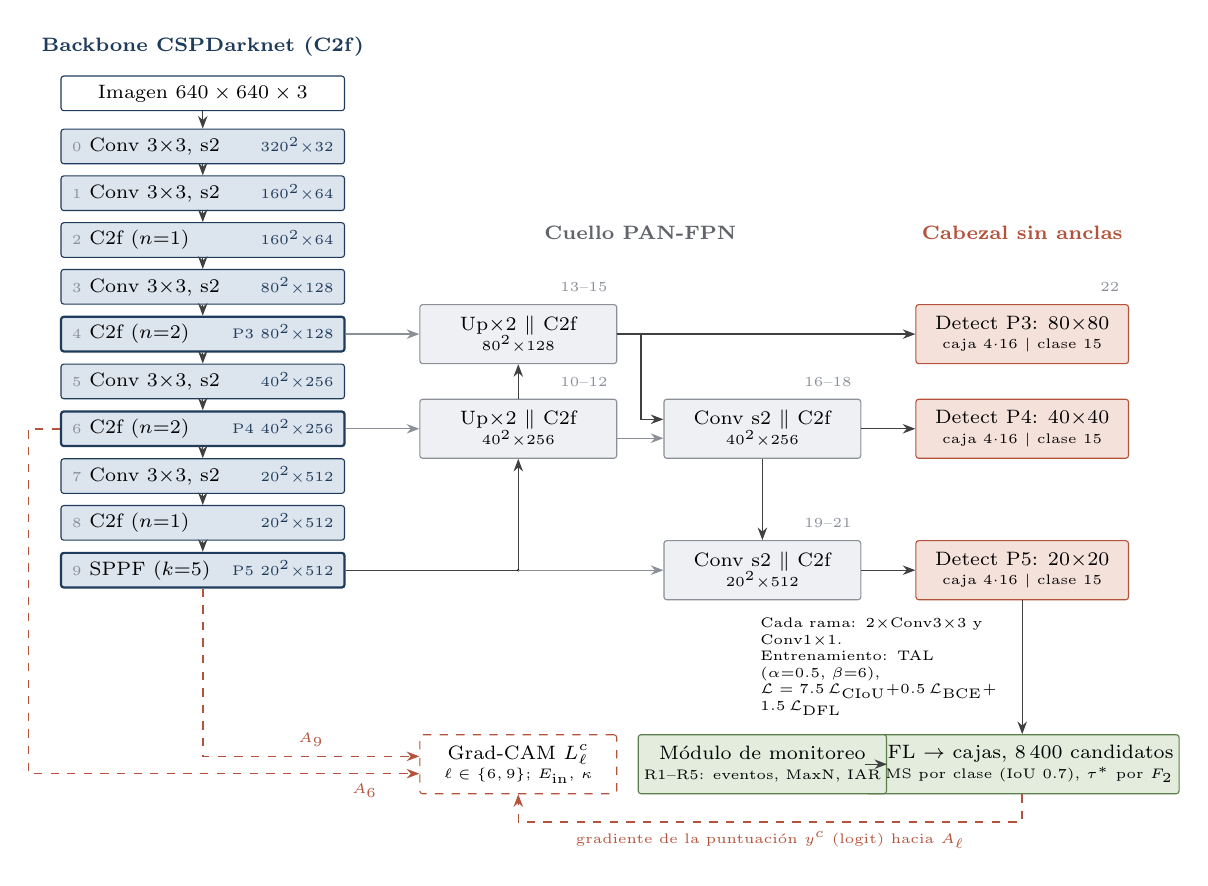
\begin{tikzpicture}[
  font=\scriptsize, >={Stealth[length=1.6mm]},
  capa/.style={draw=azul, fill=azulc, rounded corners=1pt, minimum width=36mm, minimum height=4.4mm, inner sep=1pt, line width=.4pt},
  cuello/.style={draw=gris, fill=grisc, rounded corners=1pt, minimum width=25mm, minimum height=7.5mm, inner sep=1.5pt, align=center, line width=.4pt},
  cabeza/.style={draw=oxido, fill=oxidoc, rounded corners=1pt, minimum width=27mm, minimum height=7.5mm, inner sep=1.5pt, align=center, line width=.4pt},
  post/.style={draw=verde, fill=verdec, rounded corners=1pt, minimum height=7.5mm, inner sep=2pt, align=center, line width=.4pt},
  idx/.style={font=\tiny, text=gris},
  dim/.style={font=\tiny, text=azul},
  flecha/.style={->, draw=black!75, line width=.45pt},
  salto/.style={->, draw=gris, line width=.45pt},
  cam/.style={->, draw=oxido, dashed, line width=.55pt},
]
% ---------------- Backbone ----------------
\newcommand{\bl}[3]{\makebox[2.2mm][l]{\tiny\color{gris}#1}\makebox[16mm][l]{#2}\makebox[15mm][r]{\tiny\color{azul}#3}}
\node[capa, fill=white, minimum width=36mm] (in) {Imagen $640\times640\times3$};
\node[capa, below=2.2mm of in] (b0) {\bl{0}{Conv $3{\times}3$, s2}{$320^2{\times}32$}};
\node[capa, below=1.4mm of b0] (b1) {\bl{1}{Conv $3{\times}3$, s2}{$160^2{\times}64$}};
\node[capa, below=1.4mm of b1] (b2) {\bl{2}{C2f ($n{=}1$)}{$160^2{\times}64$}};
\node[capa, below=1.4mm of b2] (b3) {\bl{3}{Conv $3{\times}3$, s2}{$80^2{\times}128$}};
\node[capa, below=1.4mm of b3, line width=.8pt] (b4) {\bl{4}{C2f ($n{=}2$)}{P3 $80^2{\times}128$}};
\node[capa, below=1.4mm of b4] (b5) {\bl{5}{Conv $3{\times}3$, s2}{$40^2{\times}256$}};
\node[capa, below=1.4mm of b5, line width=.8pt] (b6) {\bl{6}{C2f ($n{=}2$)}{P4 $40^2{\times}256$}};
\node[capa, below=1.4mm of b6] (b7) {\bl{7}{Conv $3{\times}3$, s2}{$20^2{\times}512$}};
\node[capa, below=1.4mm of b7] (b8) {\bl{8}{C2f ($n{=}1$)}{$20^2{\times}512$}};
\node[capa, below=1.4mm of b8, line width=.8pt] (b9) {\bl{9}{SPPF ($k{=}5$)}{P5 $20^2{\times}512$}};
\draw[flecha] (in) -- (b0);
\foreach \a/\b in {0/1,1/2,2/3,3/4,4/5,5/6,6/7,7/8,8/9} \draw[flecha] (b\a) -- (b\b);
\node[font=\scriptsize\bfseries, text=azul, above=1.2mm of in] {Backbone CSPDarknet (C2f)};

% ---------------- Cuello PAN-FPN ----------------
\coordinate (cx1) at ($(b0.east)+(22mm,0)$);
\coordinate (cx2) at ($(b0.east)+(53mm,0)$);
\node[cuello] (n12) at (cx1 |- b6) {Up$\times2$ $\Vert$ C2f\\[-.3mm]{\tiny$40^2{\times}256$}};
\node[cuello] (n15) at (cx1 |- b4) {Up$\times2$ $\Vert$ C2f\\[-.3mm]{\tiny$80^2{\times}128$}};
\node[cuello] (n18) at (cx2 |- b6) {Conv s2 $\Vert$ C2f\\[-.3mm]{\tiny$40^2{\times}256$}};
\node[cuello] (n21) at (cx2 |- b9) {Conv s2 $\Vert$ C2f\\[-.3mm]{\tiny$20^2{\times}512$}};
\node[idx, above=.3mm of n12.north east, anchor=south east] {10--12};
\node[idx, above=.3mm of n15.north east, anchor=south east] {13--15};
\node[idx, above=.3mm of n18.north east, anchor=south east] {16--18};
\node[idx, above=.3mm of n21.north east, anchor=south east] {19--21};
\node[font=\scriptsize\bfseries, text=gris!70!black] at ($(n15.north)!.5!(n15.north -| n18.north)+(0,9mm)$) {Cuello PAN-FPN};
% descendente (FPN), laterales y ascendente (PAN)
\draw[flecha] (b9.east) -| (n12.south);
\fill (b9.east -| n12.south) circle (.5pt);
\draw[salto] (b9.east -| n12.south) -- (n21.west);
\draw[flecha] (n12.north) -- (n15.south);
\draw[salto] (b6.east) -- (n12.west);
\draw[salto] (b4.east) -- (n15.west);
\draw[flecha] (n15.east) -- ++(3mm,0) coordinate (q15) |- ($(n18.west)+(0,1.2mm)$);
\draw[salto] ($(n12.east)+(0,-1.2mm)$) -- ($(n18.west)+(0,-1.2mm)$);
\draw[flecha] (n18.south) -- (n21.north);
% ---------------- Cabezal desacoplado ----------------
\coordinate (hx) at ($(cx2)+(33mm,0)$);
\node[cabeza] (h3) at (hx |- n15) {Detect P3: $80{\times}80$\\[-.3mm]{\tiny caja $4{\cdot}16$ $\mid$ clase 15}};
\node[cabeza] (h4) at (hx |- n18) {Detect P4: $40{\times}40$\\[-.3mm]{\tiny caja $4{\cdot}16$ $\mid$ clase 15}};
\node[cabeza] (h5) at (hx |- n21) {Detect P5: $20{\times}20$\\[-.3mm]{\tiny caja $4{\cdot}16$ $\mid$ clase 15}};
\node[idx, above=.3mm of h3.north east, anchor=south east] {22};
\node[font=\scriptsize\bfseries, text=oxido] at ($(h3.north)+(0,9mm)$) {Cabezal sin anclas};
\draw[flecha] (q15) |- (h3.west);
\draw[flecha] (n18.east) -- (h4.west);
\draw[flecha] (n21.east) -- (h5.west);
\node[font=\tiny, align=left, anchor=north east, text width=30mm] at ($(h5.south)+(-2mm,-1mm)$)
  {Cada rama: $2\times$Conv$3{\times}3$ y Conv$1{\times}1$.\\ Entrenamiento: TAL ($\alpha{=}0.5$, $\beta{=}6$),\\ $\mathcal{L}=7.5\,\mathcal{L}_{\mathrm{CIoU}}+0.5\,\mathcal{L}_{\mathrm{BCE}}+1.5\,\mathcal{L}_{\mathrm{DFL}}$};

% ---------------- Posprocesamiento ----------------
\node[post, below=17mm of h5, minimum width=27mm] (nms) {DFL $\to$ cajas, 8\,400 candidatos\\[-.3mm]{\tiny NMS por clase (IoU 0.7), $\tau^\ast$ por $F_2$}};
\draw[flecha] (h5.south) -- (nms.north);
\node[post, minimum width=27mm] (mon) at (cx2 |- nms) {Módulo de monitoreo\\[-.3mm]{\tiny R1--R5: eventos, MaxN, IAR}};
\draw[flecha] (nms.west) -- (mon.east);
% ---------------- Grad-CAM ----------------
\node[draw=oxido, dashed, rounded corners=1pt, fill=white, align=center, minimum width=25mm, minimum height=7.5mm, inner sep=2pt]
  (gc) at (cx1 |- mon) {Grad-CAM $L^c_\ell$\\[-.3mm]{\tiny $\ell\in\{6,9\}$; $E_{\mathrm{in}}$, $\kappa$}};
\draw[cam] (b9.south) -- ++(0,-3mm) coordinate (q9) |- ($(gc.west)+(0,1mm)$) node[pos=.75, above, font=\tiny, text=oxido] {$A_9$};
\draw[cam] (b6.west) -- ++(-4mm,0) |- ($(gc.west)+(0,-1.2mm)$) node[pos=.93, below, font=\tiny, text=oxido] {$A_6$};
\draw[cam] (nms.south) -- ++(0,-3.5mm) -| (gc.south) node[pos=.25, below, font=\tiny, text=oxido] {gradiente de la puntuación $y^c$ (logit) hacia $A_\ell$};
\end{tikzpicture}
\end{document}
